\documentclass[11pt]{article}

% Change "review" to "final" to generate the final (sometimes called camera-ready) version.
% Change to "preprint" to generate a non-anonymous version with page numbers.
\usepackage{acl}

% Layout and font packages
\usepackage{amsmath}
\usepackage{booktabs}
\usepackage{array}
\usepackage{microtype}
%\usepackage{inconsolata}
\usepackage{graphicx}
\graphicspath{{figures/common/}{figures/approach_1/}{figures/approach_2/}}

% Font selection for LuaLaTeX
\usepackage[english,bidi=default]{babel}
\babelfont{rm}[Extension=.otf,UprightFont=*-regular,BoldFont=*-bold,ItalicFont=*-italic,BoldItalicFont=*-bolditalic]{texgyretermes}

%%% include whatever languages you need below this line
%%% To add Indic or non-Latin languages, place the font TTF/OTF files in a fonts/ directory:
%\babelprovide[import]{hindi}
%\babelfont[*devanagari]{rm}[
%  Path = fonts/,
%  BoldFont = NotoSansDevanagari-Bold.ttf
%]{NotoSansDevanagari-Regular.ttf}

% Macro to reset title and counters between concatenated papers
\makeatletter
\AtBeginDocument{
  \let\acl@maketitle\maketitle
  \let\acl@@maketitle\@maketitle
}
\newcommand{\nextpaper}{%
  \clearpage
  \let\maketitle\acl@maketitle
  \let\@maketitle\acl@@maketitle
  \thispagestyle{empty}%
  \pagestyle{empty}%
  \setcounter{section}{0}%
  \setcounter{subsection}{0}%
  \setcounter{figure}{0}%
  \setcounter{table}{0}%
  \setcounter{equation}{0}%
}
\makeatother

\begin{document}

% -------------------------------------------------------------
% PART I: APPROACH 1
% -------------------------------------------------------------
\title{Layer-wise Isotropy of Indic Language Representations\\in Small Embedding and Generative Language Models}

\author{
  \textbf{Group: Mixture of Experts} \\
  Indian Institute of Technology Gandhinagar
}

\maketitle

\begin{abstract}
We measure how uniformly small language models use their representation space when reading 22 scheduled Indian languages and English. For every layer we compute IsoScore, average random cosine similarity, maximum explainable variance, and intrinsic dimension on token and sentence representations of the n-way parallel IN22-Gen benchmark. We compare two contrastively trained embedding models (EmbeddingGemma-300M, Qwen3-Embedding-0.6B) with two generative models (Gemma-3-1B-PT, Qwen3.5-0.8B-Base). The last transformer layer is near rank-one in most models because of a few massive activation dimensions; the final RMSNorm removes them, so isotropy must be reported before and after it. After the norm, the embedding models are more isotropic than the generative models (token IsoScore 0.23 and 0.11 against 0.04). Languages with high tokenizer fertility, such as Manipuri in Meitei script and Santali in Ol Chiki script, produce the most clustered sentence representations.
\end{abstract}

\section{Feedback and Proposed Novelty}
\label{sec:app1_feedback_novelty}

% Rubric Requirements (10 Pts):
% 1. Write the feedback provided and the novelties discussed with the mentor.
% 2. Write all feedback since Presentation 1.
% 3. Report the work completed in weekly meetings with your mentors.

\paragraph{Feedback Since Presentation 1}
% Document all feedback and action items received from the course instructors and TAs during and after Presentation 1.
[Detail the specific feedback points received after Presentation 1 here.]

\paragraph{Weekly Mentor Progress}
% Report the milestones achieved and discussions held during weekly mentor syncs.
[Summarize weekly mentor meeting discussions, adjustments made to the scope, and verified progress.]

\paragraph{Proposed Novelties}
% Explain the novel solutions and architectural or procedural modifications discussed and approved by the mentor.
[Articulate the core novelties introduced in Approach 1, why they improve upon existing methods, and how they address previous feedback.]

\section{State of the Art and Baselines}
\label{sec:app1_baselines_sota}

\paragraph{State of the Art}
\citet{ethayarajh-2019-contextual} showed that contextual representations of BERT, ELMo, and GPT-2 are anisotropic: random words have high average cosine similarity, and this grows with depth. That work introduced the average random cosine as an anisotropy baseline and maximum explainable variance (MEV) as the share of variance on the first principal component. \citet{rudman-etal-2022-isoscore} showed that average cosine and partition-based scores do not measure uniform use of dimensions and proposed IsoScore, which is 1 when variance is spread equally over all $d$ dimensions and 0 when it lies on one direction. They also used the maximum likelihood intrinsic dimension (ID) of \citet{levina-bickel-2004-maximum}. Both works study English text only.

\paragraph{Multilingual Representation Geometry}
\citet{rajaee-pilehvar-2022-isotropy} found that multilingual BERT lacks the outlier dimensions of English BERT but is still highly anisotropic, and that increasing its isotropy improves semantic similarity. They also found that the spaces of different languages are partially similar in structure. \citet{hammerl-etal-2023-exploring} studied outlier dimensions in multilingual encoders and found that sentence transformers fine-tuned on parallel data are more isotropic, which matches our embedding models. In their analysis, non-Latin scripts occupy separate regions of the space. Whitening or removing outlier dimensions after training improves cross-lingual retrieval without fine-tuning, but harms the already aligned sentence transformers. \citet{ji-etal-2023-isotropic} linked isotropy to zero-shot cross-lingual transfer and improved transfer by enhancing isotropy together with constrained code-switching. In multilingual machine translation, \citet{lai-etal-2023-mitigating} showed that tokens of low-resource languages collapse into a small subspace and used contrastive learning with target-side monolingual data to separate them. \citet{rust-etal-2021-good} showed that tokenizer quality, measured by fertility and the share of words split into several tokens, explains much of the performance gap between multilingual and monolingual models. These studies use encoders such as mBERT and XLM-R or translation models, and cover few Indic languages. We study recent small generative and embedding models on all 22 scheduled Indian languages, and relate their geometry to script and tokenizer fertility.

\paragraph{Competitive Baselines}
Our baselines are the metrics and the models. We report average random cosine and MEV \citep{ethayarajh-2019-contextual} next to IsoScore and ID \citep{rudman-etal-2022-isoscore}, so results stay comparable to both papers. Within a model family, the generative model is the baseline for the embedding model: Gemma-3-1B-PT for EmbeddingGemma-300M, and Qwen3.5-0.8B-Base for Qwen3-Embedding-0.6B. English (\texttt{eng\_Latn}) is the language baseline for the 22 Indic languages.

\paragraph{Baseline Availability}
The official IsoScore implementation is available as the \texttt{IsoScore} Python package, and \citet{rudman-etal-2022-isoscore} compute ID with \texttt{scikit-dimension}. Both are written in NumPy and run on the CPU. With 16{,}000 points per layer, up to 30 layers, 3 views, 4 models, and 23 languages, this is slow and requires copying every hidden state off the GPU. We therefore ported IsoScore (steps 2 to 7 of the paper), MEV, average random cosine, and the ID estimator to PyTorch so that they run on the GPU next to inference. A unit test checks that our IsoScore matches the official package within $10^{-6}$ on a rotated, shifted, anisotropic Gaussian. Further tests check the expected values on isotropic and rank-one data and recover the dimension of a known linear subspace.

\section{Dataset Formulation and Bias Mitigation}
\label{sec:app1_datasets}

\paragraph{Data Curation and Preprocessing}
For now we use IN22-Gen \citep{gala-etal-2023-indictrans2}, the general-domain evaluation set of IndicTrans2 (CC-BY-4.0). It has 1{,}024 sentences drawn from Wikipedia and other web sources, translated into all 22 scheduled Indian languages, together with their English source. The sentences cover 13 broad categories: culture, economy, education, entertainment, geography, government, health, industry, legal, news, religion, sports, and tourism. We use all 1{,}024 sentences for each of the 23 languages. No training split is needed because the study only runs inference.

\paragraph{Sample Bias Mitigation}
IN22-Gen is n-way parallel, so every language carries the same content. Differences between languages therefore come from script, tokenizer, and model, not from topic. The 13 categories cover general language use instead of one domain, so the samples are not biased towards a single register. For the token view, IsoScore depends on the number of points, so we draw exactly $N = 16{,}000$ tokens for every language and model. Tokens are drawn uniformly from all non-special tokens of all 1{,}024 sentences, not from the first sentences, with a seed fixed per dataset and language. Special and padding tokens are excluded from every view.

\paragraph{Bottlenecks Encountered}
Tokenizer fertility (tokens per whitespace word) varies widely. With the Gemma tokenizer, it ranges from 1.34 for English and 1.48 for Hindi to 6.36 for Santali (Ol Chiki) and 12.13 for Manipuri (Meitei), that is, from 33{,}896 to 284{,}181 tokens per language. Keeping all hidden states for such languages does not fit in memory, so the sampled token positions are fixed before inference and gathered batch by batch. Gemma models and some datasets are gated on Hugging Face and need an approved access token. At layer 0 the same token id always has the same vector, so exact duplicates are removed before estimating ID.

\paragraph{Dataset Extensions and Distinctions}
Prior isotropy studies use English corpora \citep{ethayarajh-2019-contextual,rudman-etal-2022-isoscore}. We extend the analysis to 22 Indic languages in 12 scripts with an aligned English reference. The pipeline also supports IN22-Conv, FLORES+, Sangraha Verified, IndicCorp v2, Wikipedia, and IITB IndicMonoDoc. These add conversational text, other parallel text, and native monolingual text, which will separate translation effects from language effects in later runs.

\section{Experimental Plan and Architecture}
\label{sec:app1_experimental_plan}

\paragraph{Experimental Setting and Robustness}
The study is inference-only. No model is trained or fine-tuned, so the geometry we measure is that of the released weights. Each model is loaded once in float32 on one GPU, and all 1{,}024 sentences of each language are run in batches of 32 with right padding. Inputs are truncated only at the model's own limit. Every hidden state is kept: the embedding output, each layer, and, for models with a final RMSNorm, the last layer both before and after that norm. We study three views per layer: $N = 16{,}000$ sampled tokens, one mean-pooled vector per sentence, and one last-token vector per sentence. We ran the following command once per model, where omitting \texttt{--langs} selects all 22 Indic languages and \texttt{--english} adds the English baseline:

\noindent
\begin{small}
\begin{verbatim}
nohup python run.py --device cuda:0 \
  --models <model> --datasets in22-gen \
  --english --n-tokens 16000 --plot \
  --overwrite --debug \
  > logs/<model>-in22-gen.log 2>&1 &
\end{verbatim}
\end{small}
Several measures keep results robust under limited compute. The same $N$ and seed are used for every language and model. Token positions are drawn before inference, so the full token matrix is never stored. All metrics run on the GPU one layer at a time. Each run saves a \texttt{run\_config.json} with all settings and library versions, refuses to mix results made with different settings, and resumes without recomputing finished languages. We report means and standard deviations over the 23 languages.

\paragraph{Models and Parameters}
We use four models: two embedding models and two generative models, one of each from the Gemma and Qwen families (Table~\ref{tab:app1_models}). The approaches differ in training objective and attention. The embedding models are trained contrastively for sentence similarity, whereas the generative models are trained only for next-token prediction. EmbeddingGemma uses bidirectional attention and mean pooling \citep{vera-etal-2025-embeddinggemma}. Qwen3-Embedding is a causal model with last-token pooling \citep{zhang-etal-2025-qwen3embedding}. Gemma-3-1B-PT uses causal attention with five sliding-window layers per global layer \citep{gemmateam-2025-gemma3}. Qwen3.5-0.8B-Base is a hybrid model in which three Gated DeltaNet linear-attention layers alternate with one full-attention layer \citep{qwenteam-2026-qwen35}. We analyse its text backbone and discard the vision encoder. Parameter counts come from the released safetensors files.

\begin{table}[t]
\centering
\small
\begin{tabular}{lrrr}
\toprule
Model & Params & $L$ & $d$ \\
\midrule
EmbeddingGemma-300M & 303M & 24 & 768 \\
Qwen3-Embedding-0.6B & 596M & 28 & 1024 \\
\midrule
Gemma-3-1B-PT & 1000M & 26 & 1152 \\
Qwen3.5-0.8B-Base & 752M & 24 & 1024 \\
\bottomrule
\end{tabular}
\caption{Models used: embedding models (top) and generative models (bottom). Params counts the transformer backbone with tied embeddings. EmbeddingGemma has 308M with its dense projection head, and Qwen3.5 has 873M with its vision encoder and multi-token prediction head. $L$ is the number of layers and $d$ the hidden size.}
\label{tab:app1_models}
\end{table}

\paragraph{Hyperparameters and Ablation Study}
No parameters are learned, so there is no grid search. The analysis settings are fixed to keep runs comparable. $N = 16{,}000$ is below the token count of every language for every tokenizer, so no language is skipped. ID uses $k = 20$ neighbours, the \texttt{scikit-dimension} default used by \citet{rudman-etal-2022-isoscore}. Average cosine uses $10^6$ random pairs. The seed is 0. Our ablation varies the representation instead: the pooling view and the position relative to the final norm. Table~\ref{tab:app1_ablation} shows that the final norm changes the conclusions more than any other setting.

\begin{table}[t]
\centering
\small
\begin{tabular}{llrrrr}
\toprule
 & & \multicolumn{2}{c}{IsoScore} & \multicolumn{2}{c}{Avg. cosine} \\
Model & View & pre & post & pre & post \\
\midrule
EmbGemma & token & .000 & .228 & .969 & .140 \\
 & mean & .001 & .190 & .999 & .557 \\
 & last & .000 & .004 & .986 & .718 \\
\midrule
Qwen3-Emb & token & .016 & .114 & .254 & .197 \\
 & mean & .034 & .067 & .825 & .760 \\
 & last & .080 & .081 & .664 & .446 \\
\midrule
Qwen3.5 & token & .019 & .038 & .549 & .550 \\
 & mean & .014 & .023 & .941 & .943 \\
 & last & .021 & .024 & .910 & .908 \\
\bottomrule
\end{tabular}
\caption{Ablation over view and final norm: last layer before (pre) and after (post) the final RMSNorm, averaged over 23 languages. The Gemma-3-1B-PT run predates the pre/post split and is omitted.}
\label{tab:app1_ablation}
\end{table}

\paragraph{Evaluation Metrics}
IsoScore is the primary metric because it is the only one among those used here that measures how evenly variance is spread over all dimensions and is invariant to rotation and scale \citep{rudman-etal-2022-isoscore}. Average random cosine and MEV are kept for comparability with \citet{ethayarajh-2019-contextual}. However, MEV on raw vectors is dominated by a few tokens with very large norms. ID separates ``variance on few directions'' from ``points on a low-dimensional manifold''. Beyond these metrics, we added three diagnostics. First, MEV on unit-length vectors counts every token equally. Second, we report the last layer before and after the final norm. Third, a norm breakdown splits RMSNorm into the per-token division and the learned per-dimension gain $\gamma$, applies each part alone, and identifies the massive dimensions. We also record tokenizer fertility for each language.

\paragraph{System Effort and Viva Demonstration}
One model on 23 languages takes a single GPU run. The 1B-parameter model in float32 needs about 4\,GB for weights. Each model produces about 130\,MB of results. For the viva, we will run the command above for EmbeddingGemma-300M on Hindi and English, show the progress log, and open the per-layer \texttt{metrics.csv}, the metric-versus-depth plot, and the 3-D PCA scatter of every layer. We will then rerun the command to show that finished languages are skipped. Finally, we will run the norm-breakdown script to show the massive dimension and its removal by $\gamma$, and compare the four models with Figure~\ref{fig:app1_depth}.

\section{Implementation Status and Preliminary Findings}
\label{sec:app1_implementation_findings}

\paragraph{Codebase Repository}
The code, run configurations, and results for Approach 1 are public:

\noindent\url{https://github.com/Ninjacoder-vedant/NLP-assignment-2-approach-1}

\paragraph{Pipeline Readiness}
The pipeline is complete from data to plots. Datasets, model families, and metrics are registered classes, so a new one is added without changing the runner. \texttt{dataset\_loader.py} downloads, caches, and aligns seven datasets. \texttt{model\_loader.py} wraps sentence-transformers and Hugging Face models behind one interface and detects the final norm. \texttt{inference.py} extracts all hidden states and the three views. \texttt{isotropy\_metrics.py} holds the GPU metrics. \texttt{run.py} runs and resumes experiments, and \texttt{plotting.py} draws per-layer metric and 3-D PCA plots. Unit tests cover the metrics and an end-to-end smoke run. Results are complete for EmbeddingGemma-300M, Qwen3-Embedding-0.6B, and Qwen3.5-0.8B-Base on all 23 languages of IN22-Gen. Gemma-3-1B-PT has a token-view run on Hindi from an earlier pipeline version.

\begin{figure}[t]
\centering
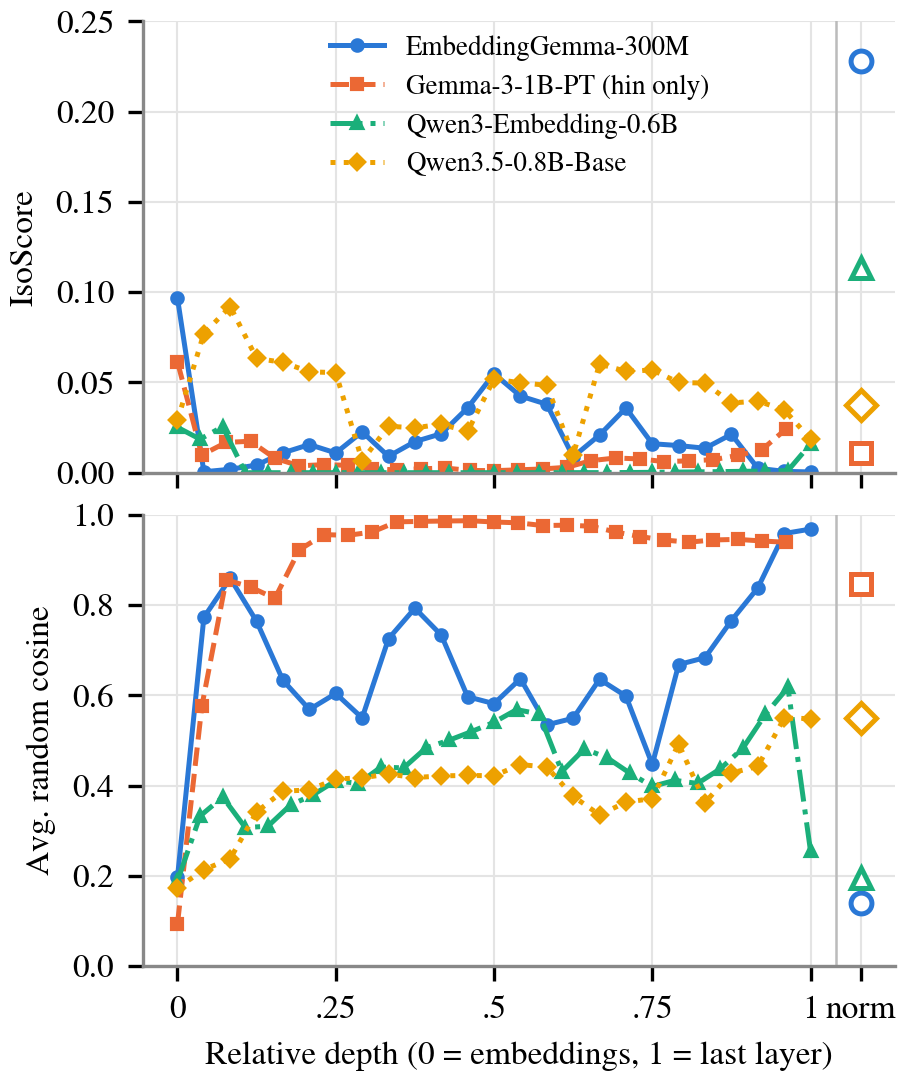
\includegraphics[width=\columnwidth]{token_isotropy_depth.png}
\caption{Token-view IsoScore and average random cosine against relative depth, averaged over 23 languages (Gemma-3-1B-PT: Hindi only). Hollow markers show the last layer after the final norm.}
\label{fig:app1_depth}
\end{figure}

\paragraph{Preliminary Findings and Result Patterns}
Figure~\ref{fig:app1_depth} and Table~\ref{tab:app1_ablation} show four patterns.

First, the last layer before the final norm is close to rank one, and the norm removes this. Before the norm, EmbeddingGemma has token IsoScore 0.000 and average cosine 0.969. After the norm, these are 0.228 and 0.140. The norm breakdown on Hindi explains this. One dimension (731) reaches about 156{,}000 in every token, against about 7{,}000 for the next largest. The learned gain $\gamma$ of this dimension is 0.23 against a median of 10.7. Applying $\gamma$ alone lowers average cosine from 0.96 to 0.10, while the per-token division alone raises IsoScore from 0.0005 to 0.16. Qwen3-Embedding removes its massive dimension (35) earlier. Its last layer's update points against the shared direction (cosine $-0.93$), so average cosine falls from 0.66 to 0.21 before the norm. Isotropy reported only at \texttt{last\_hidden\_state} hides this behaviour.

Second, after the norm, embedding models are more isotropic than generative models. Token IsoScore is 0.228 for EmbeddingGemma and 0.114 for Qwen3-Embedding, against 0.038 for Qwen3.5-Base and 0.011 for Gemma-3-1B-PT on Hindi. Average cosine follows the same order: 0.14 and 0.20 against 0.55 and 0.85. Mean-pooled sentence IsoScore is 0.190 and 0.067 against 0.023. Contrastive training spreads the output space, which matches its use for similarity search.

Third, the inner layers behave differently across families. In Qwen3-Embedding, layers 3 to 16 have MEV above 0.99 and IsoScore near 0, because massive activations hold almost all variance. In Qwen3.5-Base, inner IsoScore stays mostly between 0.02 and 0.09 and MEV near 0.1, except at layers 7 and 15, where MEV rises to 0.35 and 0.29. In Gemma-3-1B-PT, average cosine stays above 0.94 from layer 8 onwards. ID drops from 18 to 35 at the embedding layer to below 5 after the first layer in every model, and stays below 20 in all later layers, far below $d$.

Fourth, languages with high fertility produce more clustered sentence representations. English has the lowest mean-pooled average cosine in all three fully run models (0.39, 0.54, 0.65). Manipuri (Meitei) and Santali (Ol Chiki) have the highest (up to 0.99), together with the lowest mean-pooled IsoScore in EmbeddingGemma and Qwen3-Embedding. With fertility from the Gemma tokenizer, the Spearman correlation between fertility and mean-pooled IsoScore is $-0.80$ for EmbeddingGemma, $-0.41$ for Qwen3-Embedding, and $-0.61$ for Qwen3.5-Base. These geometric patterns describe the representation space and do not by themselves measure task quality.

\paragraph{Limitations}
The Gemma-3-1B-PT result covers only Hindi and comes from an earlier pipeline version without the pre-norm split. The Qwen pair differs in generation (Qwen3 against Qwen3.5) as well as objective. All results use one dataset, one $N$, and one seed. IN22-Gen sentences are translated from English, so translation effects are not yet separated from language effects.

\section{Computational Resources and Project Management}
\label{sec:app1_resources_management}

\subsection{Conception of Novel Solutions}
We started from the isotropy literature \citep{ethayarajh-2019-contextual,rudman-etal-2022-isoscore}, which studies English text with older encoders. Two gaps followed: no study covers the scripts and tokenization levels of Indian languages, and no study compares a contrastive embedding model with a generative model of the same family. Early runs showed a sharp change in every metric at the final norm, so we added the pre/post-norm split and the norm breakdown to the method.

\subsection{Computational Environment}
Table~\ref{tab:app1_compute_resources} lists the resources used. The study needs one GPU at a time. Several models can run in parallel on separate GPUs with \texttt{--device}.

\begin{table}[t]
\centering
\small
\begin{tabular}{l>{\raggedright\arraybackslash}p{3.6cm}}
\toprule
Resource Component & Specification \\
\midrule
Hardware Accelerator & [GPU model] \\
GPU Video Memory & [VRAM]; float32 weights need 1.2 to 4.0\,GB \\
System Memory (RAM) & [RAM] \\
CPU Cores & [cores] \\
Persistent Storage & About 130\,MB of results per model, plus model weights and dataset cache \\
Software Stack & Python, PyTorch 2.10 to 2.11, Transformers 5.16 to 5.18, sentence-transformers 5.4 to 5.7, Datasets 4.8 to 5.0 \\
\bottomrule
\end{tabular}
\caption{Computational resources and environment for Approach 1.}
\label{tab:app1_compute_resources}
\end{table}

\subsection{Task Distribution and Workflow}
% TODO: fill in who did what for Approach 1.
[Detail the breakdown of responsibilities and workflow distribution among the team members assigned to Approach 1.]


% -------------------------------------------------------------
% PART II: APPROACH 2
% -------------------------------------------------------------
\nextpaper

\title{[Approach 2 Title: Specific Title of Second Work]}

\author{
  \textbf{Group: Mixture of Experts} \\
  Indian Institute of Technology Gandhinagar
}

\maketitle

\begin{abstract}
% State the specific research problem, core methodology, key novelty, and empirical findings for Approach 2.
This paper presents Approach 2 for CS 613: Natural Language Processing Assignment 2. We investigate [insert core concept of Approach 2]. We detail mentor feedback received, baseline models, dataset curation and bias mitigation strategies, the experimental architecture, and preliminary implementation progress.
\end{abstract}

\section{Feedback and Proposed Novelty}
\label{sec:app2_feedback_novelty}

% Rubric Requirements (10 Pts):
% 1. Write the feedback provided and the novelties discussed with the mentor.
% 2. Write all feedback since Presentation 1.
% 3. Report the work completed in weekly meetings with your mentors.

\paragraph{Feedback Since Presentation 1}
% Document all feedback and action items received from the course instructors and TAs during and after Presentation 1.
[Detail the specific feedback points received after Presentation 1 for Approach 2 here.]

\paragraph{Weekly Mentor Progress}
% Report the milestones achieved and discussions held during weekly mentor syncs.
[Summarize weekly mentor meeting discussions, adjustments made to the scope, and verified progress.]

\paragraph{Proposed Novelties}
% Explain the novel solutions and architectural or procedural modifications discussed and approved by the mentor.
[Articulate the core novelties introduced in Approach 2, why they improve upon existing methods, and how they address previous feedback.]

\section{State of the Art and Baselines}
\label{sec:app2_baselines_sota}

% Rubric Requirements (10 Pts):
% 1. Report the other baselines you want to compete with.
% 2. What is the state-of-the-art (the best paper that has solved the approach)?
% 3. Are baseline implementations available for the novelties?

\paragraph{State of the Art}
% Identify and discuss the strongest published paper and benchmark that addresses this task.
[Cite and describe the current state of the art paper that achieves leading performance on this problem. Explain its key techniques and limitations.]

\paragraph{Competitive Baselines}
% List the baseline models selected for empirical comparison and explain why they were chosen.
[Describe the baseline architectures and algorithms selected for benchmarking against Approach 2.]

\paragraph{Baseline Availability}
% Clarify whether official or reliable third-party open-source implementations exist for these baselines or if custom implementations are required.
[State whether open-source implementations are available for the baselines and novel components, citing repositories or describing custom re-implementations.]

\section{Dataset Formulation and Bias Mitigation}
\label{sec:app2_datasets}

% Rubric Requirements (05 Pts):
% 1. How did you tackle the bias in your samples?
% 2. What bottleneck did you encounter?
% 3. How did you extend the existing dataset, and what are the differences between it and the previous one?

\paragraph{Data Curation and Preprocessing}
% Detail the primary datasets used, split sizes (train, validation, test), and token distributions.
[Describe the origin, domain, and characteristics of the raw dataset used in Approach 2.]

\paragraph{Sample Bias Mitigation}
% Discuss identified selection, representation, or demographic biases in the data and the steps taken to counteract them.
[Explain the specific analytical or algorithmic strategies employed to identify and mitigate sample bias in the dataset.]

\paragraph{Bottlenecks Encountered}
% Document data constraints, cleaning difficulties, alignment issues, or missing labels faced during preparation.
[Detail data-level bottlenecks encountered during curation, such as high noise levels, class imbalance, or token length constraints.]

\paragraph{Dataset Extensions and Distinctions}
% If the dataset was augmented or extended, describe how it differs quantitatively and qualitatively from the original baseline benchmark.
[Describe how the dataset was extended or modified compared to standard benchmarks, explicitly highlighting structural and distributional differences.]

\section{Experimental Plan and Architecture}
\label{sec:app2_experimental_plan}

% Rubric Requirements (15 Pts):
% 1. Experimental setting, training procedures, and robustness under limited computational resources.
% 2. Models used, architectural differences, and computed parameter counts.
% 3. Hyperparameter search techniques (grid search or better techniques).
% 4. Ablation table with different hyperparameters.
% 5. Metric selection rationale and additional metrics explored.
% 6. System effort required and scenario for the final viva demonstration.

\paragraph{Training Setup and Robustness}
% Describe training hardware constraints, precision settings, batching, optimizer choice, and techniques used to ensure stable results (e.g., cross-validation, multiple seeds).
[Describe the experimental environment, training configuration, and measures taken to ensure empirical robustness given compute bounds.]

\paragraph{Architectures and Parameters}
% List the model variants used, provide exact parameter counts, and articulate the key architectural modifications that distinguish them.
[Detail model architectures, parameter counts, and structural modifications distinguishing this approach from baselines.]

\paragraph{Hyperparameter Optimization and Ablation Study}
% Describe the hyperparameter search method (e.g., grid search, Bayesian optimization) and summarize performance across configurations in Table~\ref{tab:app2_ablation}.
[Explain how optimal hyperparameters were determined across algorithms and baselines.]

\begin{table*}[t]
\centering
\small
\begin{tabular}{lcccc}
\toprule
Configuration & Learning Rate & Batch Size & Primary Metric & Secondary Metric \\
\midrule
Baseline & $1 \times 10^{-4}$ & 16 & 0.00 & 0.00 \\
Variant A & $5 \times 10^{-5}$ & 32 & 0.00 & 0.00 \\
Variant B & $2 \times 10^{-5}$ & 32 & 0.00 & 0.00 \\
Full Model & $2 \times 10^{-5}$ & 64 & 0.00 & 0.00 \\
\bottomrule
\end{tabular}
\caption{Hyperparameter ablation study for Approach 2.}
\label{tab:app2_ablation}
\end{table*}

\paragraph{Evaluation Metrics}
% Justify primary metrics chosen and discuss any exploratory or complementary metrics evaluated.
[Justify the primary evaluation metrics selected and describe any secondary or non-standard metrics tested.]

\paragraph{Viva Demonstration Scenario}
% Paint a clear, concrete walkthrough of what will be demonstrated interactively to course examiners during the viva.
[Provide an end-to-end scenario demonstrating user input, model inference, and output inspection during the viva session.]

\section{Implementation Status and Preliminary Findings}
\label{sec:app2_implementation_findings}

% Rubric Requirements (50 Pts Implementation + 10 Pts Findings):
% 1. Codebase repository link.
% 2. Boiler code readiness across dataset preparation, training, and evaluation pipelines.
% 3. Reporting patterns in preliminary results and findings for smaller LLMs and baselines.

\paragraph{Codebase Repository}
% Provide the direct GitHub repository link containing the code for Approach 2.
The source code, configuration files, and replication scripts for Approach 2 are maintained at:
\url{https://github.com/[org-or-user]/[approach-2-repo]}

\paragraph{Pipeline Readiness}
% Describe implementation milestones: data cleaning, tokenization, training loop, validation checkpoints, and inference scripts.
[Detail the modular structure of the pipeline, confirming that data preparation, training, and evaluation scripts are functional.]

\paragraph{Preliminary Findings and Result Patterns}
% Report patterns observed in initial baseline runs on smaller models (e.g., convergence behaviors, common failure modes, initial metric comparisons).
[Discuss the preliminary empirical findings and emerging result patterns observed across initial smaller model experiments.]

\section{Computational Resources and Project Management}
\label{sec:app2_resources_management}

% Rubric Requirements (10 Pts):
% 1. How did you manage to propose the novel solutions?
% 2. Computational resources needed (RAM, GPUs, CPU Cores, Hard Disk, etc.).
% 3. Project division and task distribution amongst group members.

\subsection{Conception of Novel Solutions}
% Describe the collaborative research process, literature review methodology, and mentor consultations that led to Approach 2's solutions.
[Explain the collaborative research process, literature review methodology, and mentor consultations that led to the proposed solutions for Approach 2.]

\subsection{Computational Environment}
% Specify hardware and infrastructure allocated for model training, inference, and fine-tuning.
Table~\ref{tab:app2_compute_resources} outlines the computational specifications utilized for our experiments.

\begin{table}[t]
\centering
\small
\begin{tabular}{l>{\raggedright\arraybackslash}p{3.6cm}}
\toprule
Resource Component & Specification \\
\midrule
Hardware Accelerator & [e.g., NVIDIA A100 / RTX 4090] \\
GPU Video Memory & [e.g., 24 GB / 40 GB VRAM] \\
System Memory (RAM) & [e.g., 32 GB / 64 GB RAM] \\
CPU Cores & [e.g., 16 virtual cores] \\
Persistent Storage & [e.g., 500 GB NVMe SSD] \\
Software Stack & PyTorch, Hugging Face, CUDA \\
\bottomrule
\end{tabular}
\caption{Summary of computational resources and environment specifications for Approach 2.}
\label{tab:app2_compute_resources}
\end{table}

\subsection{Task Distribution and Workflow}
% Outline the operational workflow and task ownership among the Approach 2 team members.
[Detail the breakdown of responsibilities and workflow distribution among the team members assigned to Approach 2.]


% -------------------------------------------------------------
% COMBINED TEAM CONTRIBUTION AND BIBLIOGRAPHY
% -------------------------------------------------------------
\clearpage
\section*{Team Contribution}
\label{sec:team_contribution}

% Rubric Requirements:
% Dedicated section at the end of the report indicating the specific contributions of all 8 group members.

Table~\ref{tab:team_contribution} summarizes the core responsibilities and execution tasks delivered by each member across both approaches.

\begin{table*}[t]
\centering
\small
\begin{tabular}{lll>{\raggedright\arraybackslash}p{6.4cm}}
\toprule
Name & Roll Number & Sub-team & Key Responsibilities \\
\midrule
Vedant Acharya & 23110010 & [Approach 1 / 2] & [e.g., Dataset curation, preprocessing pipeline, baseline evaluation] \\
Chavda Haarit Ravindrakumar & 23110077 & [Approach 1 / 2] & [e.g., Model architecture design, training scripts, ablation studies] \\
Darpana Dharmesh Desai & 23110085 & [Approach 1 / 2] & [e.g., Bias mitigation, data filtering, exploratory metric analysis] \\
Devansh Lodha & 23110091 & [Approach 1 / 2] & [e.g., Pipeline implementation, hyperparameter search, report drafting] \\
Jagtap Arnav Shrikant & 23110143 & [Approach 1 / 2] & [e.g., State-of-the-art benchmarking, training loop development] \\
Suhani & 24110358 & [Approach 1 / 2] & [e.g., Data augmentation, evaluation scripts, viva demo design] \\
Keval Pintubhai Shah & 26120003 & [Approach 1 / 2] & [e.g., Computational resource setup, baseline reproducibility] \\
Ruddhi Pintubhai Shah & 26250038 & [Approach 1 / 2] & [e.g., Qualitative error analysis, result visualization, documentation] \\
\bottomrule
\end{tabular}
\caption{Detailed breakdown of individual responsibilities and project contributions across all group members.}
\label{tab:team_contribution}
\end{table*}


\nocite{*}
\bibliography{references}

\end{document}
